\chapter{总结和展望}

\section{工作总结}

预测着色器程序在不同平台的性能对于游戏开发等需要高实时性的场合具有比较重大的意义。对此,本文首先在第二章简要介绍了绘制流水线、着色器等基础知识,同时回顾了着色器程序优化、程序语言理解和性能建模三个方面的工作。因为绘制流水线环节相对复杂,GPU 厂商种类和架构多种多样,着色器作为领域专用的程序语言本身,其层次较高,与最后的 GPU 原生指令存在较大差距。故而,本研究受相关工作启发,设计了{\amend 面向性能预测的着色器性能数据集,以及}数据驱动的、基于 SPIR-V 和 Transformer 进行平台独立的性能预测的{\amend 着色器性能预测模型}。

本研究收集了在 5 种平台上运行 Shadertoy 网站的着色器程序形成的着色器性能数据集,并对数据集的质量和内容进行了一定程度的评估{\added ,进行了挑战样本集切分,并同时探究了使用基座语言模型进行着色器类型标注的相关方法。}在{\amend 第四章}设计性能模型时,本研究着重考虑了多种因素。为了保证平台无关性,本方法选择只使用应用程序呈递给图形 API 的信息;为了复用已有的工具链,同时兼顾网络的学习效果和平台独立的特性,本方法选择使用 SPIR-V 作为预测模型的输入;为了提升模型预测的表现,克服图灵完备的着色器程序性能预测问题中理论和实际的困难,本方法选择加入 SPIR-V 指令计数信息,并用基本块为粒度进行指令编排和追踪运行。以上的设计考虑给模型的预测精度和方法本身的泛用性之间取得了不错的平衡。

本研究提出的方法在测试的所有平台上均取得了不错的效果,同基线方法相比均有一定程度的提升。特别的,本研究利用消融和对比实验,验证了指令计数追踪、指令嵌入生成和数据归一化方面的实践是相对优秀的。

\section{未来展望}

% 1. Performance measurement problem as whole
%    - 不同于其他领域,软件工程中的性能是较少被理解的。
%    - 部分原因:
%      1) 性能进步很快,Moore's Law;
%      2) 软件层次上的复杂性 %%,以及第一性原理的缺乏
%      3) 快速变化的需求
% 2. 解决性能问题的第一步是了解性能
%    - 将性能知识以更易得的手段得以分发
%    - 端到端,这样面对复杂系统时候才可能测量出其中的损耗
% 3. 本文工作可以被视为是“构造复杂处理器系统上的性能基线”的一部分
%    - NPU,GPU,CPU - 设计能力、制造能力都影响性能
%    - 但是对于给定的任务,最优的设计是什么样的?软件的峰值性能可以反馈硬件的迭代和设计
% 4. 本文工作的缺陷
%    - 数据集 bias (类别和分布)
%    - 准确性缺陷
%    - 可解释性缺陷
%    - scope 缺陷
% 5. 从本文工作延伸开去,性能需要更多的为人所理解;优化的第一步也是了解性能。希望这里的工作可以向这里迈进一步。

% 理解计算机系统上运行的各类应用程序的性能是一个颇有挑战性的课题。在土木工程中,建造师可以通过标准化的、查询图纸、定额的方式,来得到整个工程基本精确的花销、耗时。但是,在软件工程领域中,大多数软件工程师在软件写完并开始运行前,都无法比较准确的估计软件预期的性能。同时,假使软件在某个平台慢了一倍两倍,恐怕绝大多数人也没法敏感的察觉——毕竟,我们也不知道一个软件应该多快。对此,多数人都有一种得过且过的心态:只要不是太慢,那就“能用就行”。在笔者看来,这种现状的形成有着多方面的原因。

理解计算机系统上运行的各类应用程序的性能是一个颇具挑战性的课题。在土木工程领域,建造师可以通过标准化的方式,查询图纸和定额,从而较为精确地估算整个工程的成本和工期。然而,在软件工程领域,大多数软件工程师在软件开发完成并开始运行之前,难以准确估计软件的预期性能。同时,如果软件在某个平台上的运行速度减慢一倍或两倍,{\amend 因为缺乏对软件应有性能的认知},大多数人也难以敏感地察觉。笔者认为,导致这种现状的形成有着多方面的原因。

% https://foxsen.github.io/archbase/%E8%AE%A1%E7%AE%97%E6%9C%BA%E7%B3%BB%E7%BB%9F%E6%80%A7%E8%83%BD%E8%AF%84%E4%BB%B7%E4%B8%8E%E6%80%A7%E8%83%BD%E5%88%86%E6%9E%90.html

其一,计算系统的性能进步曾经很快。Intel 公司的创始人 Gordon Moore 曾经提出摩尔定律:芯片上的晶体管每两年就要翻一番 \cite{MooreLaw}。特别是在 CPU 单核性能进步的“黄金时期”,编写的程序可以很轻松的收到处理器工艺和设计进步带来的红利,无需进行软件性能优化即可随时间获得客观的性能提升。图 \ref{fig:specint} 中 1985 年到 2004 年左右的时期即体现了这一趋势,此时基本表征单核性能的 SPECint 分数依指数增长。

其二,软件和硬件的层次都在逐渐增多,让理解性能变得更加困难。相较于 20 年前,现在的 CPU 增加了更多的缓存级别、更丰富的专用指令、更多层次的并行粒度,现在的操作系统增加了更多的功能、更复杂的多核调度,现在的程序设计语言和相应的函数库也增加了更多高层级的特性,同时系统中可能还会出现 GPGPU、NPU 等加速芯片。这些额外的层次都使得理解性能本身的难度变得更高。

其三,快速变化的需求让节约程序编写时长产生的收益超越了优化程序运行时间所产生的收益。例如在敏捷开发方法中,主要强调快速响应变化和持续交付的价值,这样开发团队可能会优先考虑编写新功能和修复错误,而不是深入优化程序的运行时间,以允许团队更快地交付新功能,从而更好地满足客户需求和市场变化。

然而,摩尔定律预言的工艺进步不是无限的。例如,从图 \ref{fig:specint} 中可以看出,从 2004 年以后,单核性能和时钟频率的增长趋于停滞,而 CPU 上运行的应用程序的性能进步主要来源于多核技术的引入。类似 CPU 的对称多处理器技术与 GPGPU、NPU 等加速器系统的出现,使得具有针对性的工作负载实现了实现更高的计算效率。但是,上述的性能提升不再是对程序员透明的,而是需要程序员在程序的设计阶段就积极考虑对目标平台和架构的适配。故而,架构优化和性能调优等工作都需要程序员对于性能有比较深入的了解。对此,笔者认为,只有让更多人以更简单的方法了解自己程序在各种不同的计算平台上的最终性能,才可以在更大程度上推动这一趋势,挖掘软硬件中被浪费的性能。构造复杂计算系统上的性能基线即是这样一种手段。

\begin{figure}
    \centering
    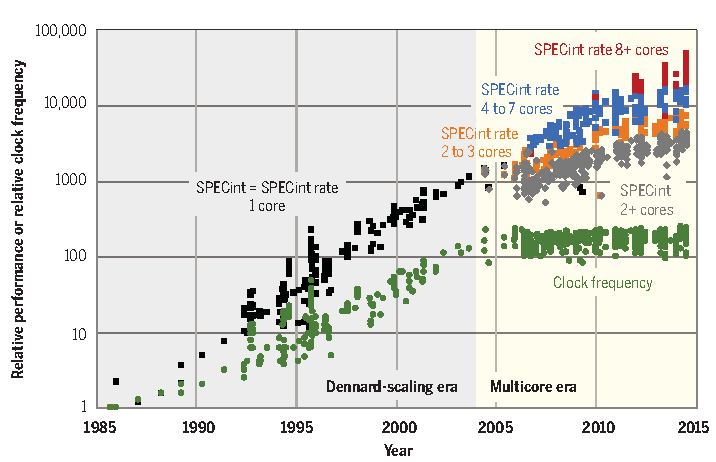
\includegraphics{figures/SPECint.pdf}
    \caption{SPECint、SPECint-rate 以及时钟频率的年际增长 \cite{doi:10.1126/science.aam9744}}
    \label{fig:specint}
\end{figure}

诚然,本研究提出的方法还有诸多不足。

其一,本研究在数据集和其相关评估过程方面存在一些局限性。虽然笔者相信本研究提出的框架具有普遍性,但截至目前,本研究只在不涉及纹理采样或多通道着色的片段着色器上验证了提出的方法。此外,本研究采用的、从Shadertoy收集的、用于验证本研究所提出方法的着色器,其可能和游戏等图形应用程序中的着色器在性能表现上有一定偏差。未来的工作中,如果能将性能测量和预测的框架进行小幅修改,以拓展到其它着色器类型(如顶点着色器、几何着色器甚至计算着色器等)的话,本研究提出的方法的普适性将会更上一个台阶。同时,为了降低和游戏等更广泛的图形程序中的着色器程序的性能特征偏差,如果将类似的着色器通过抓帧的方法截取和记录,并且收集整理成为数据集的话,将对着色器性能的理解有不小的帮助。在着色器之外,固定管线资源和其它和性能相关的因素也可以进一步加入讨论,以创建一个完整的、端到端的绘制和计算流水线黑盒性能模型。

其二,本研究的准确性仍然有进步空间。鉴于本研究收集到的性能数据,其变异系数均在3\%以下,故而本研究提出的预测器的准确性在理论上仍然有一定的改进空间。正如第 \ref{sec:challenge} 节所讨论的,有许多因素影响着着色器程序的性能。这些因素来自方方面面,并且可能会以相互交织的形式共同影响最终的性能表现。这样一来,当前采集的性能样本,其数量可能不足以充分训练本研究提出的模型。笔者认为,数据增强可能是一种可行的解决手段。例如,通过对着色器中的表达式进行有损失的强度削弱、或通过 IR 变换的方法首先对着色器进行变异,再使用变异后的变体来进行性能样本的增强,可能可以暴露更多对理解性能起到帮助的性能样本,并让本研究提出的模型训练的更加出色。此外,在 SPIR-V 指令追踪阶段,当前的指令追踪方法只记录了着色器程序全部线程调用后的总指令执行数目。如果将这里的记录方式变为逐线程记录的话,虽然指令追踪阶段的速度会大大下降,且可能面临存储和使用上的困难,但是这些额外的信息很可能可以帮助模型更好的挖掘线程之间影响性能的行为。这也是一种更细粒度的性能上下文信息。另一种提升模型性能表现的思路是,通过跨语言的通用展示来提升待构造的着色器性能模型的表现。类似 GraphCodeBERT \cite{DBLP:conf/iclr/GuoRLFT0ZDSFTDC21}的预训练范式在本研究的工作中尚没有得到应用,但利用在其它语言上训练好的通用程序语言表示,再加以着色器专有的性能任务进行微调的方法,未尝不是一种可能的选择。

其三,作为数据驱动的方法,性能预测的可解释性仍然需要更多关注。具体到本研究,虽然本研究提出的预测模型能够以平台独立的方式,针对目标平台上运行的着色器程序提供相对准确的性能预测值,但是确定该着色器性能现状的瓶颈的问题仍然需要程序员自身的智慧。对此,笔者认为可行的一种改进是构造或实现一类在各个典型性能瓶颈方向上变异的着色器性能样本对,并在程序员需要优化建议时,通过让本研究提出的模型预测这些变化后的着色器的时间,来给出大致的瓶颈方向的参考。

除了以上这些局限之外,最近非常活跃的大语言模型领域也启发笔者,本研究提出的方法可能可以作为将性能数据加入解决程序任务的大模型中的一种方法。一种可能的想法是,通过将性能信息送入经过预训练的大模型中,这些大模型可能拥有以完全自动化的方式优化用户提供的着色器、并且解决用户所面临的软件性能问题的能力。